\documentclass{article}
\usepackage{graphicx} % Required for inserting images
\usepackage{kotex}
\usepackage{amsmath}
\usepackage{mathtools}
\usepackage{amssymb}
\usepackage{amsthm}
\usepackage[margin=2cm,nonhead]{geometry}
\usepackage{setspace}   
\usepackage{abstract}
\usepackage{authblk}
\usepackage{enumitem}

\newtheorem{thm}{Theorem}
\theoremstyle{definition}
\newtheorem{defn}[thm]{Definition}
\theoremstyle{theorem}
\newtheorem{theorem}{Theorem}
\theoremstyle{proposition}
\newtheorem{prop}{Proposition}
\theoremstyle{corollary}
\newtheorem*{corol}{Corollary}



\onehalfspacing
\setlength\parindent{0pt}


\renewcommand\Affilfont{\small}

\title{\textbf{Minimal Grid Diagrams of Theta-Curves and Handcuff Graphs up to 7 Crossings}}
\author[1]{Eunchan Cho}
\author[1]{Jeongwon Shin}
\author[1]{Boyeon Seo}
\author[1]{Minho Choi}
\author[2]{Hun Kim}
\author[3]{Gyotaek Jin}
\affil[1]{Researcher, Korea Scinece Academy of KAIST}
\affil[2]{Supervisor, Korea Science Academy of KAIST}
\affil[3]{Co-Supervisor, Department of Mathematical Sciences, Korea Advanced Institute of Scienceand Technology}


\renewcommand\Authands{ and }

\date{\vspace{-5ex}}

\begin{document}



\begin{center}
    {\LARGE \textbf{엇갈림수 7 이하의 세타 커브와 핸드커프 그래프의 최소 그물그림}\par}
    \vspace{0.3cm}
    {\large 조은찬\textsuperscript{1}, 신정원\textsuperscript{1}, 서보연\textsuperscript{1}, 최민호\textsuperscript{1}, 김훈\textsuperscript{2}, 진교택\textsuperscript{3}}\\
    {\large \textsuperscript{1}연구자, 한국과학영재학교 \par \textsuperscript{2}책임지도자, 한국과학영재학교 \par \textsuperscript{3}공동지도자, 한국과학기술원 수리과학과\par}

    \renewenvironment{abstract}
    {\begin{quote}
    \noindent \rule{\linewidth}{.5pt}\par{\bfseries \abstractname.}}
    {\medskip\noindent \rule{\linewidth}{.5pt}
    \end{quote}
    }

    \renewcommand{\abstractname}{초록}


    \begin{abstract}
        한글 한 글 하 ㄴ 글 한ㄱ ㅡㄹ 한 글 한글\\
        \textbf{중심어 : theta-curve, handcuff graph, arc index, Yamada polynomial}
        \\
    \end{abstract}

    \vspace{1cm} % 한글/영문 사이 간격

    {\LARGE \textbf{Minimal Grid Diagrams of Theta-Curves and Handcuff Graphs up to 7 Crossings}\par}
    \vspace{0.3cm}
    {\large Eunchan Cho\textsuperscript{1}, Jeongwon Shin\textsuperscript{1}, Boyeon Seo\textsuperscript{1}, Minho Choi\textsuperscript{1}, Hun Kim\textsuperscript{2}, Gyotaek Jin\textsuperscript{3}}\\
    {\large \textsuperscript{1}Researcher, Korea Science Academy of KAIST \par \textsuperscript{2}Supervisor, Korea Science Academy of KAIST\par \textsuperscript{3}Co-Supervisor, Department of Mathematical Sciences, Korea Advanced Institute of Science and Technology}
\end{center}

\renewenvironment{abstract}
{\begin{quote}
\noindent \rule{\linewidth}{.5pt}\par{\bfseries \abstractname.}}
{\medskip\noindent \rule{\linewidth}{.5pt}
\end{quote}
}

\begin{abstract}
본 연구에서는 공간 그래프(spatial graph), 특히 엇갈림 수(crossing number) $7$까지의 $\theta$-곡선($\theta$-curve)과 수갑 그래프(handcuff graph)에서의 최소 격자 그래프(minimal grid diagram)을 구함으로써 그들의 호 지수(arc index)를 확정시키고자 하였다. 또한 그 과정에서 호 지수의 상한과 하한을 구할 수 있었으며, 야마다 다항식(yamada polynomial)을 통해 파이썬 프로그램을 작성하여 이를 확인해 보닸다.  
    \\ \\
\textbf{Keywords : theta-curve, handcuff graph, arc index, Yamada polynomial}
\\
\end{abstract}


\begin{abstract}
Our purpose of this research is classifying theta-curves and handcuff graphs by their arc indices, which their crossing is up to 7.
We tried to find those arc indices by proving lower bounds and upper bounds of the theta-curves and handcuff graphs.
Also we programmed Python code that returns Cromwell matrix of the theta curves which have crossing up to 7.
Yamada polynomial was used to prove bounds and programming the Python code.\\ \\
\textbf{Keywords : theta-curve, handcuff graph, arc index, Yamada polynomial}
\\
\end{abstract}


\section{Introduction}
Knot theory is a field of mathematics that studies simple closed curves embedded in three-dimensional space.
Study of theta-curves and handcuff graphs is included in knot theory.
In this research, we tried to classify those graphs by their arc indices, which are up to 7 crossings.\\


We first decided to used the Python code to examine the arc index.
For this, we found the method classifying theta-curve and handcuff graphs by Cromwell matrix.
Finding all possible matrices for those graphs and finding out the Yamada polynomial of each graphs could give the minimal arc index of the graph, but the Topoly library of the Python did not work, so we could not examine the Yamada polynomial.
So, we found out the smallest Cromwell matrix by hand with using the bounds of the arc index, and used the Python code to examine if we found the right Cromwell matrices.
Then we tried to decrease the gap of upper and lower bounds, and found out arc indices of some graphs.

\section{Theoretical Background}


\textit{Theta-curve} is a spatial knot on 3-sphere which has 2 vertices and 3 edges. In the projection of the theta-curve, the section where theta-curve meets itself is named \textit{crossing}. If the one theta-curve and other theta-curve's continuous transform of the graph is same, these curves are \textit{equivalent}. To transform a projection of theta-curve, the \textit{generalized Reidemeister move} is used.\\

\textit{Handcuff graph} consists of two loops and an edge joining the loops. In the projection of the handcuff graph, the section where handcuff graph meets itself is named \textit{crossing}. If the one handcuff graph and other handcuff graph's continuous transform of the graph is same, these graphs are \textit{equivalent}. Similar with the theta-curve, the \textit{generalized Reidemeister move} is used to transfrom a projection of handcuff graph.\\

\begin{figure*}[h]
    \centerline{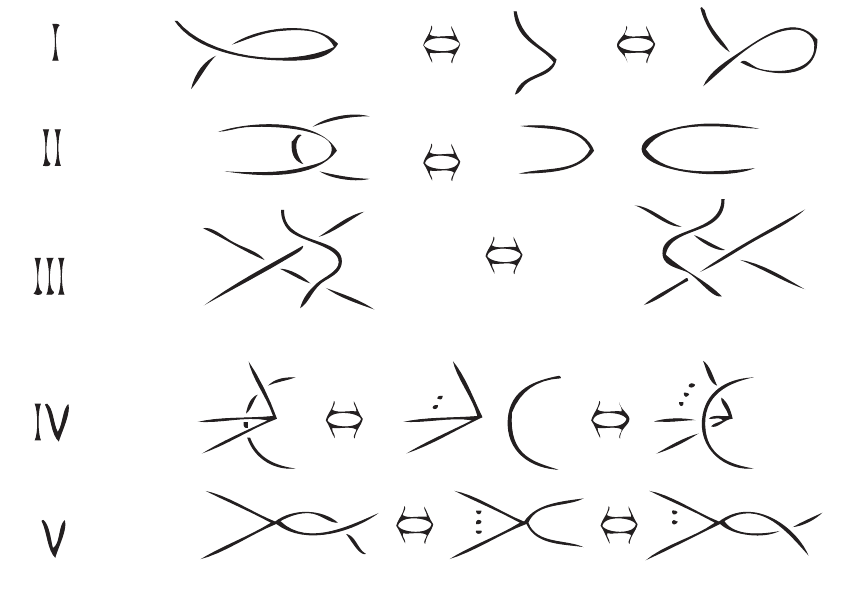
\includegraphics[width=0.5\textwidth]{generalized_reidemeister.png}}
    \caption{Generalized Reidemeister moves.}
    \label{figure_1} 
\end{figure*}

\textit{Arc presentation} is an open-book decomposition of $\mathbb{R}^3$ which has open half-planes as pages and the standard z-axis as the binding axis. Every spatial graph $G$ can be embedded in an open-book decomposition with finitely many pages so that it meets each page in exactly one simple arc with two different end-points on the binding axis.
In knot theory, \textit{arc index}, is the minimal number of pages among all possible arc presentations of graph. This arc presentation with the minimal number of pages is \textit{minimal arc presentation.} \textit{Prime knots} are knots that is not constructed by combining simpler knots. We are finding the arc index for the prime theta-curve and handcuff graph up to seven crossings.\\

The \textit{grid diagram} is a handcuff graph or theta‐curve diagram of vertical strands and one less number of horizontal strands with the properties that at every crossing the vertical strand crosses over the horizontal strand and no two horizontal segments are co‐linear and no two vertical segments are co‐linear.
The \textit{Cromwell matrix} is an $n \times n$ binary matrix each of whose rows and columns has exactly two 1s. For theta‐curve and handcuff graph, its Cromwell matrix is an $n \times (n+1)$ binary matrix that exactly two rows (called Three‐rows) has exactly three 1s and rest of the rows and each columns has exactly two 1s.
If the 1s are connected by horizontal and vertical lines, it leads to the grid diagram. The arc presentation can be expressed by grid diagram and vice versa. They are in one-to-one correspondence. Also, if the number of half planes are $\alpha$ on minimal arc presentation, the size of corresponding grid diagram is $(\alpha - 1) \times \alpha$.\\

\begin{figure*}[h]
    \centerline{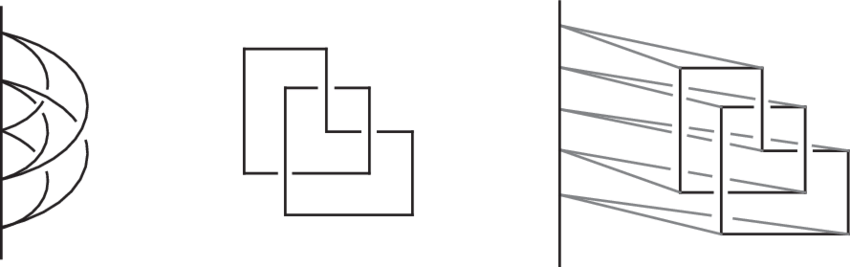
\includegraphics[width=0.5\linewidth]{An arc presentation and a grid diagram of the knot.png}}
    \caption{An arc presentation and a grid diagram of the knot}
    \label{figure_2}
\end{figure*}

The \textit{link with $n$-components} is an embedding of the disjoint union of $n$ circles $S^1 \cup \cdots \cup S^1$ in $\mathbb{R}^3$. $1$-component link is called a \textit{knot}. The $\theta$-curve 아귀찮아 이건 나중에\\

The polynomial of the knot is invariant. \textit{Yamada polynomial} is invariant when it is mulitplied $(-x)^n$ for some integer n. The \textit{span} of a knot, is substraction of maximal degree of minimal degree of the polynomial. It is a invariant since Yamada polynomial is invariant when mulitplied by $(-x)^n$.\\

\begin{figure*}[h]
    \centerline{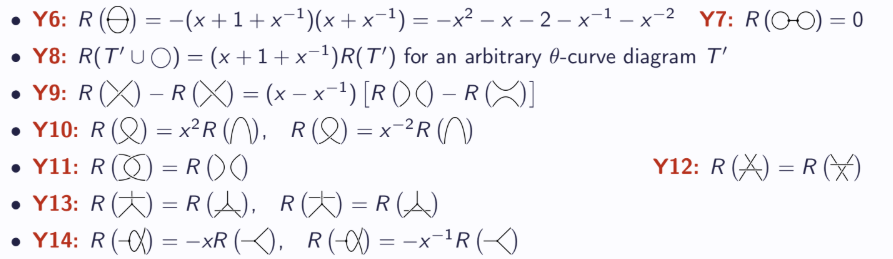
\includegraphics[width=0.75\linewidth]{yamada_property.png}}
    \caption{Properties of Yamada polynomial.}
    \label{figure_3}
\end{figure*}

Let 3 edges of theta-curve is $e_1, e_2, e_3$, then $e_1 \cup e_2$, $e_2 \cup e_3$, $e_3 \cup e_1$ becomes a knot on 3-sphere. This knots are \textit{consituent knot} of the theta-curve.

\textit{Stacked tangle} of an theta-curve is stacked disks each with the frame as boundary with following properties:
\begin{itemize}
\item Only two disk called \textit{non-simple disks} contain one vertex and three line
segments which joins the vertex and boundary point.
\item One of the non-simple disks is at the top.
\item Other disks called \textit{simple disks} contain simple arc which joins two
points on the boundary.
\item When view from above
\begin{itemize}
    \item two arcs in different simple disks intersect at most one point (by RII)
    \item arc in simple disk and tree in non-simple disk intersect at most one
point (by RV)
\end{itemize}
\end{itemize}

\textit{Simple closure} of stacked tangle is a stacked tangle with \textit{caps} satisfying following properties:
\begin{itemize}
    \item A \textit{cap} is a simple arc in outside of stacked tangle joining end points of arcs or line segments
    \item When view from above any tow caps have no intersection.
\end{itemize}
Then a simple closure of a stacked tangle without any nested caps is
corresponding to an arc presentation.\\

A \textit{reduced simple closure of a stacked tangle} is
\begin{itemize}
    \item a simple closure of a stacked tangle without any nested caps
    \item any two arcs(including line segment) joining by caps have no intersection when view from above
\end{itemize}

\subsection{Lower bounds of Arc Index in Theta-Curve}

\begin{theorem}
Let T be any theta-curve and $K_1$, $K_2$, $K_3$ be three constituent knots of T. Then $$\alpha(T) \geq \underset{i \in \{1,2,3\}}\max \alpha(K_i) + 1.$$
\end{theorem}

\begin{theorem}
Let T be any theta-curve and $K_1$, $K_2$, $K_3$ be three constituent knots of T. Then $$\alpha(T) \geq \frac{1}{2}\sum_{i=1}^3\alpha(K_i).$$
\end{theorem}

\begin{theorem}
For any theta-curve $\theta$, $$\alpha(\theta)\geq\frac{1+\sqrt{f(\alpha(\theta))+36c(\theta)}}{3} \left(f(x) = \begin{cases} 
		73 & x \equiv 0 \pmod 6\\ 
		4 & x \equiv 1 \pmod 6\\ 
		25 & x \equiv 2 \pmod 6\\ 
		-8 & x \equiv 3 \pmod 6\\ 
		49 & x \equiv 4 \pmod 6\\ 
		20 & x \equiv 5 \pmod 6\\ 
     \end{cases} \right).$$
\end{theorem}

\begin{theorem}
Let T be any theta-curve. Then $$2+\sqrt{\max\deg_x R(S_T) - \min\deg_x R(S_T) + 4} \leq \alpha(T)$$ where $R(T)$ is a Yamada polynomial of the theta-curve T, and $S_{T}$ be a reduce simple closure of stacked tangle of a theta-curve T corresponding to minimal arc presentation of T.
\end{theorem}

\subsection{Upper bound of Arc Index in Theta-Curve}

\begin{theorem}
For theta-curve $\theta$, if $c(\theta)$ is the minimal crossing number, then $$\alpha(\theta) \leq c(\theta) + 3.$$
\end{theorem}

\begin{proof}
$$\alpha(\theta) \leq c(\theta) + e + b$$ when e is number of edges, b is number of bouquet cut-components. We have 3 edges, 0 bouquet cut-componentes for theta-curves. Therefore, $$\alpha(\theta) \leq c(\theta) + 3.$$
\end{proof}

\section{Research Methods and Procedure}
First, we made a Python Code to find the arc index and the cromwell matrix of the knots. Then we used the upper and lower bounds, and also found the smaller upper bounds and larger lower bounds. Finally we used the direct method to find the arc index by drawing the binding circle.

\subsection{The Python Code(가제)}
The Python Code(가제) generates the possible Cromwell matrix of theta-curves, and compares with the existing knots in the table which is less or equal to 7 crossings.
It eventually returns the Cromwell matrix of the compared theta-curve.
To distinguish the Cromwell matrices from theta-curves and handcuff graphs, which is generated and removed by the rules from the above section, we should use the determinant of the Cromwell matrices.\\

\begin{defn}
The \textit{grid diagram} of a knot is a projection that consists only of horizontal and vertical lines, and the vertical line always passes above the horizontal line. (However, in this case, there must be exactly two points (excluding the vertices) that are vertically bent for each horizontal line (row) and vertical line (column), and the two vertices must be on the horizontal line.)
\end{defn}
\begin{defn}
The \textit{THC-Cromwell matrix} is the matrix that satisfies the following conditions.
\end{defn}
\begin{enumerate}
    \item It is a $n\times(n+1)$ matrix with entries 0 and 1.
    \item It has only two `1's in every row and column, except for two rows. These two rows have three `1's.
\end{enumerate}
\begin{theorem}
Every theta-curve and handcuff graph has its corresponding THC-Cromwell matrix.
\end{theorem}
$\mathbf{Definition}$ Let any exception row(with three `1's) $i$ and its two outer `1's $j$, $k$. The \textit{H-deletion Matrix} of THC-Cromwell matrix is $(n-1)\times(n-1)$ matrix which deleted row $i$ and column $j$, $k$.\\

\subsubsection{Main Theorem}
\begin{theorem}The given THC-Cromwell matrix is theta-curve if and only if determinant of the H-deletion matrix is $\pm 1$.The given THC-Cromwell matrix is handcuff graph if and only if determinant of the H-deletion matrix is 0 or $\pm 2$.
\end{theorem}

\begin{proof}
\begin{enumerate}
    \item \textbf{Method of changing grid diagram of a knot to simple matrix}\\
    First, we should change grid diagram of a knot into Cromwell matrix. However, we can apply row operation of interchanging the rows. In this way, determinant of the Cromwell matrix would change only by multiplying $\pm 1$.\\
By applying row operation, we should make matrix such as
    $$\begin{pmatrix} 
    1 & 1 & 0 & \cdots & 0\\
    0 & 1 & 1 &  &  \\
    0 & 0 & 1 & & \vdots\\ 
    \vdots & & & \ddots & \\
    1 & 0 & \cdots & 0 & 1
    \end{pmatrix}$$
Let matrix is $n\times n$.
Next, we apply the row operation. We add the upper rows to the most bottom row. Then,
    $$\begin{pmatrix} 
    1 & 1 & 0 & \cdots & 0\\
    0 & 1 & 1 &  &  \\
    0 & 0 & 1 & & \vdots\\ 
    \vdots & & & \ddots & \\
    2 & 2 & \cdots & 2 & 2
    \end{pmatrix}$$
Lastly, by subtracting ($2i-1$)th row $(i \in \mathbb{N})$ with multiplying row by 2 and substract with most bottom row, if n is even, the most bottom row only contains 0. Since it is upper triangular matrix, we can obtain determinant by trace. Hence the last entry is 0, the determinant is 0. If n is odd, the last entry of most bottom row is 2 and other entry is all 0. Since it is upper triangular matrix, we can obtain determinant by trace too. Hence the other entry is all 1, the determinant is $\pm 2$.\\

\item \textbf{Proof in the case of theta-curve}\\
Do the H-deletion. Then, we can make the matrix of this grid diagram by previous section. If end vertices is erased when we delete the row, then by what vertices is erased in the other three vertices row in the grid diagram can make different matrix.
\begin{enumerate}
    \item \textbf{0}\\
    T-shaped figure is given.
    \item \textbf{1 (middle vertex)}\\
    Line-shaped figure is given.
    \item \textbf{1 (end vertex)}\\
    Line-shaped figure is given.
    \item \textbf{2 (two end vertices)}\\
    T-shaped figure is given.
    \item \textbf{2 (middle and end vertices)}\\
    Line-shaped figure is given.
\end{enumerate}

\begin{enumerate}[label={(\roman*)}]
    \item \textbf{Line-shaped figure}\\
    Let the matrix is given.
    $$\begin{pmatrix}
        1 & 1 & 1 & 0\\
        0 & 1 & 1 & 1\\
        1 & 0 & 0 & 1
    \end{pmatrix}$$
    If you work on deleting rows and columns here, you can get the line-shaped figure of the following figure. If you convert this into a matrix according to the previous section,
    $$\begin{pmatrix}
        1 & 1 \\
        0 & 1
    \end{pmatrix}$$
    is given.\\
    If we appropriately perform adding multiple of one row to another row and replacing the second row with the result, the determinant changes only by $\pm 1$, and the resulting matrix will be identity matrix. If we appropriately transform other theta-curves, we can get the same result.
    \item \textbf{T-shaped figure}\\
    Let the matrix is given.
    $$\begin{pmatrix}
        1 & 1 & 1\\
        1 & 1 & 1\\
    \end{pmatrix}$$
    If you work on deleting rows and columns here, you can get the T-shaped figure of the following figure. If you convert this into a matrix according to the previous section,
    $$\begin{pmatrix}
        1 & 1 & 1\\
        0 & 1 & 0\\
        0 & 0 & 1
    \end{pmatrix}$$
    is given.\\
    If we appropriately perform adding multiple of one row to another row and replacing the second row with the result, the determinant changes only by $\pm 1$, and the resulting matrix will be identity matrix. If we appropriately transform other theta-curves, we can get the same result.
\end{enumerate}
Therefore, $\pm 1$ will be the determinant of the theta-curve's H-deletion matrix.

\item \textbf{Proof in the case of handcuff graph}\\
    Do the H-deletion. Then, we can make the matrix of this grid diagram by upper section. If end vertices is erased when we delete the row, then by what vertices is erased in the other three vertices row in the grid diagram can make different matrix.
    \begin{enumerate}
        \item \textbf{0}\\
        Knot is given.
        \item \textbf{1 (middle vertex)}\\
        Line-shaped figure is given.
        \item \textbf{1 (end vertex)}\\
        It is not given since one column might have 3 vertices.
        \item \textbf{2 (two end vertices)}\\
        It is not given since rows which have 3 vertices is connected with 2 line.
        \item \textbf{2 (middle and end vertices)}\\
        It is not given since rows which have 3 vertices is connected with 2 line.
    \end{enumerate}
    
    \begin{enumerate}[label={(\roman*)}]
        \item \textbf{Knot}\\
        By upper section, the determinant becomes 0 or $\pm 2$.
        \item \textbf{Line-shaped figure}
        Let the matrix is given.
        $$\begin{pmatrix}
            0 & 0 & 0 & 1 & 1\\
            0 & 1 & 0 & 1 & 1\\
            1 & 1 & 1 & 0 & 0\\
            1 & 0 & 1 & 0 & 0
        \end{pmatrix}$$
        If you work on deleting rows and columns here, you can get the line-shaped figure of the following figure. If you convert this into a matrix according to the previous section,
        $$\begin{pmatrix}
            1 & 1 & 0 \\
            0 & 1 & 1 \\
            0 & 0 & 0 \\
        \end{pmatrix}$$
        Since it is upper triangular matrix, the determinant of the matrix is trace, so the determinant of this matrix is 0.
    \end{enumerate}
\end{enumerate}
\end{proof}

\subsection{Bounds of Arc Index in case of Theta-Curves}
We used the bounds from theoretical background, and used the Python code to find the arc index. If we could not find the arc index by the computer, we directly found the arc index by drawing the binding circle of the theta-curve.

\subsection{Bounds of Arc Index in case of Handcuff Graphs}

\begin{defn}
    The \textit{non-simple cap} is the cap that connects simple disk and non-simple disk or two non-simple disks.
\end{defn}

\begin{theorem}
The number of the simple cap of the graph $G$ is invariant if least one of the edges are not crossed with others when the projection has minimal crossing, except the trivial theta-curve.
\end{theorem}
\begin{proof}
     To find the number of the non-simple cap from the grid diagram, we can draw the horizontal lines which include 1 from row that has three 1s. Since non-simple cap connects 1s from rows which have three 1s, the number of horizontal lines is the number of the non-simple caps. When the edge that directly connects two vertices is not crossed, the number of edges that starts from the vertices, which is 5, is the number of the horizontal lines. It can be shown by drawing the binding circle of the knot. Since the binding circle crosses the crossed area of two other edges, the number of edges that starts from the vertices is 5, 2 from each vertices and 1 that directly connects the vertices, except the trivial theta-curve. Since $\alpha(G))$ is the number of caps, the number of simple cap is $\alpha(G) - 5$.\\
\end{proof}

\begin{defn}
    In a handcuff curve, the \textit{vertex edge} is an edge that is connected to both vertices.
\end{defn}

\begin{defn}
    In a handcuff curve, the \textit{link component} is a union of the loops from each vertex to itself.
\end{defn}

\begin{theorem}[뭐시기뭐시기 출처모름]
    If $L$ is an alternating and non-split link, then
    \[ \alpha(L) = c(L)+2. \]
    %crossing number 정의를 써야하나???
\end{theorem}

\begin{theorem}[뭐시기뭐시기 출처모름]
    For any spatial graph $H$,
    \[ \alpha(H) \leq c(H)+e+b, \]
    where $e$ is the number of the edge and $b$ is the number of the bouquet.
\end{theorem}

\begin{corol}
    If $H$ is a handcuff curve,
    \[ \alpha(H) \leq c(H)+5. \]
    Especially, if the link component of $H$ is non-split,
    \[ \alpha(H) \leq c(H)+3. \]
\end{corol}

\begin{proof}
    If $H$ is a handcuff curve, the number of the edge is $3$, and the number of the bouquet is at most $2$. Thus the first inequality holds since $e=3, b \leq 2$. If there is a bouquet, one of the loops can be pulled out without affecting the rest. (See figure 1.) Then, if we remove the vertex edge of $H$, the remaining link component is a split link. Thus there are no bouquet if the link component of $H$ is non-split, and we have second inequality since $e=3, b=0$.
\end{proof}

\begin{figure*}
    \centerline{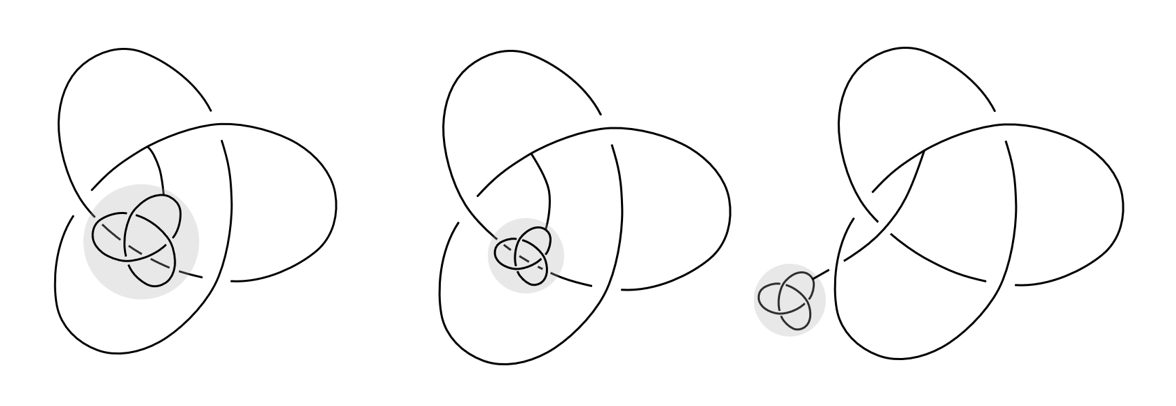
\includegraphics[width=\textwidth]{image.png}}
    \caption{caption}
    \label{figure_4} 
\end{figure*}

\begin{prop}
    For a handcuff curve $H$, let $L$ be a link component of $H$. Then,
    \[ \alpha(H) \geq \alpha(L)+1. \]
\end{prop}
\begin{proof}
    In the arc presentation of $H$, let $v_1$, $v_2$ be the vertices of $H$. Then, there are half-planes that contain the vertex edge of $H$. If we remove them, the remainder is the arc presentation of $L$, the link component of $H$. Since the number of half-planes that contain the vertex edge is at least $1$, we obtain
    \[ \alpha(H) \geq \alpha(L) + (\text{the number of half plane that contain vertex edge}) \geq \alpha(L)+1. \]
\end{proof}

Using the Theorem 1, we obtain the following corollary.

\begin{corol}
    In the handcuff curve, if the link component $L$ is alternating and non-split, then
    \[ \alpha(H) \geq c(L)+3. \]
\end{corol}

Combining the above corollary and the corollary of Theorem 2, we have the following theorem.

\begin{theorem}
    For the handcuff curve $H$, if the link component $L$ is alternating and non-split, then
    \[ \alpha(H) = c(L)+3. \]
\end{theorem}

\begin{theorem}
    뭐시기 출처 모름
\end{theorem}
\begin{theorem}
    뭐시기 출처 모름
\end{theorem}


\section{Research Result}
The Python Code did not work since the Topoly Library had error of the Yamada polynomial function. However, we were able to examine some of our answers by the Python Code. Also, we were able to found the bounds of the arc index of the handcuff graphs.


\section{Conclusion}
요약, 더 나아가서 어떻게 써먹을 수 있을지?

\begin{thebibliography}{9}
    \bibitem{lamport94}
    Leslie Lamport.
    \newblock \LaTeX: A Document Preparation System.
    \newblock Addison Wesley, Reading, Massachusetts, second edition, 1994.
    
    \bibitem{knuth84}
    Donald E. Knuth.
    \newblock The \TeX book.
    \newblock Addison Wesley, Reading, Massachusetts, 1984.
\end{thebibliography}


\end{document}